\documentclass{article}
\usepackage{graphicx} % Required for inserting images
\usepackage{ctex}
\usepackage{listings}

\title{NPUcore}
\author{Flame Star}
\date{May 2024}

\renewcommand*{\thefigure}{5-\arabic{figure}}

\begin{document}

\maketitle

\section{NPUcore特性}
\subsection{内存管理方面}
\subsubsection{页表与地址空间管理}
在 NPUcore-Impact!!! 中,虚拟地址空间和物理地址空间均采用页式管理,且每个页面的大小为 4KiB (2^{12}B).

对于页表以及地址的管理可参见下表.\\

\begin{center}
\begin{tabular}{|c|c|c|c|}
\hline
地址 & 页号 & 页内偏移 & 总位数 \\
\hline
虚拟地址VA & VPN-38:12 27bit & Offset-11:0 12bit & 39bit \\
物理地址PA & VPN-55:12 44bit & Offset-11:0 12bit & 56bit \\
\hline
\end{tabular}
\\

表5-1:地址详细列表

\end{center}
\subsubsection{地址的数据结构抽象}
\begin{center}
\begin{lstlisting}[language=RUST,numbers=left]
#[repr(C)]
#[derive(Copy, Clone, Ord, PartialOrd , Eq, PartialEq)]
pub struct PhysAddr(pub usize);

#[repr(C)]
#[derive(Copy, Clone, Ord, PartialOrd , Eq, PartialEq)]
pub struct VirtAddr(pub usize);

#[repr(C)]
#[derive(Copy, Clone, Ord, PartialOrd , Eq, PartialEq)]
pub struct PhysPageNum(pub usize);

#[repr(C)]
#[derive(Copy, Clone, Ord, PartialOrd , Eq, PartialEq)]
pub struct VirtPageNum(pub usize);
\end{lstlisting}

代码5-1:存储地址数据结构
\end{center}

上面分别给出了物理地址 PA、虚拟地址 VA、物理页号 PPN、虚拟页号 VPN 的类型声明,它们都是元组式结构体,可以看成 usize 的一种简单包装。我们刻意将它们各自抽象出不同的类型而不是都使用与 RISC-V 64 硬件直接对应的 usize 基本类型,是为了在 Rust 编译器的帮助下,通过多种安全且方便的类型转换来构建页表.

\subsubsection{页表项}

\begin{figure}[h]
    \centering
    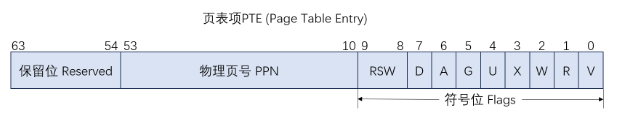
\includegraphics[width=1\linewidth]{figs\PTE.PNG}
    \caption{页表项的格式}
    \label{P}
\end{figure}

其中,对于符号位的详细解释如下:

\begin{itemize}
    \item V(Valid):有效位。仅当 V 为 1 时,该页表项合法;
    \item R(Read)/W(Write)/X(eXecute):分别表示索引到这个页表项的对应虚拟页面是否允许读/写/执行;
    \item U(User):表示索引到这个页表项的对应虚拟页面是否在 CPU 处于 U 特权级的情况下允许访问;
    \item G(Global):全局标志。为 1 时表明该页面为全局页面;
    \item A(Accessed):处理器使用此位来记录自页表项上的这一位被清零后,其对应虚拟页面是否被访问过;
    \item D(Dirty):处理器使用此位来记录自页表项上的这一位被清零后,其对应虚拟页面是否被修改过;
    \item RSW(Reserved for Supervisor softWare):保留位。该部分被处理器忽略,软件可以使用.
\end{itemize}

\subsubsection{地址空间}
内核地址空间有四个标志位,具体为
\begin{center}
\textbf{\textit{R - 读;W - 写;X - 执行;U - 用户.}}
\end{center}
\\
\textbf{\textit{对于内核程序区域而言:}}

在\textbf{os/src/linker.in.ld}下,我们可以找到对应的基址,其值为:
\begin{center}
    \textbf{0x0000000090000000}.
\end{center}

而对于本次新的开发板LoongArch-2k1000而言,其MMIO区域并无多少设备,仅有一UART寄存器,具体可在\textbf{os/src/arch/la64/board/2k1000.rs}下找到UART寄存器地址:

\begin{center}
    \textbf{0x1fe20000}.
\end{center}

目前仅介绍了部分重要地址,由于更换开发板,大部分地址常数已经重写,具体可参见\textbf{os/src/arch/la64/config.rs},将于附于本章文末.

\subsection{进程调度方面}
对于进程调度,NPUcore-Impact!!!给出了一系列方法用于提升操作系统的性能.
\newpage
\subsubsection{进程生命周期}
对于NPUcore-Impact!!!的进城生命周期,我们给出下图以使读者有直观了解.

\begin{figure}[htb]
    \centering
    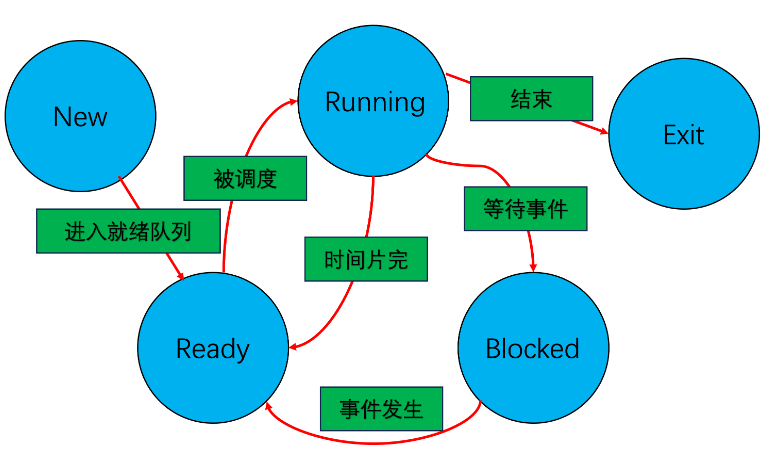
\includegraphics[width=1\linewidth]{figs\Proc.PNG}
    \caption{进城生命周期示意图}
    \label{fig:enter-label}
\end{figure}

NPUcore-Impact!!!团队在进行性能优化时,发现在操作系统运行示例程序时,IO 操作导致CPU 挂起的性能损失非常之大,因此我们将调度器进行了大改,使其完全支持了阻塞式的进程调度模式,即构建挂起队列,使进程不能获得资源时可被挂起,直到满足可操作的条件后再进行操作.

\subsubsection{资源复用}

\begin{center}
\begin{tabular}{|c|c|}
    \hline
    内核 & NPUcore-Impact!!!\\
    单核/多核 & 单核 \\
    \hline
    资源复用思路 & 一段所有进程共享的跳板代码+一个进程的私有的保存现场的帧\\
    资源回收思路 & 释放一部分资源等待父进程完成剩下资源回收\\
    \hline
    进程管理方式 & TCB* \\
    \hline
\end{tabular}
表5-2:NPUcore-Impact!!!的复用思路
\end{center}

这里我们引出NPUcore-Impact!!!特殊的一点——TCB(TaskControlBlock/任务控制块):不同于传统的 PCB 数据结构,npucore
将线程视为共享栈的进程.

\begin{center}
\begin{lstlisting}[language=RUST,numbers=left]
pub struct TaskControlBlock {
    // immutable
    pub pid: PidHandle ,
    pub tid: usize,
    pub tgid: usize,
    pub kstack: KernelStack ,
    pub ustack_base: usize,
    pub exit_signal: Signals ,
    // mutable
    inner: Mutex<TaskControlBlockInner >,
    // shareable and mutable
    pub exe: Arc<Mutex<FileDescriptor >>,
    pub tid_allocator: Arc<Mutex<RecycleAllocator >>,
    pub files: Arc<Mutex<FdTable >>,
    pub fs: Arc<Mutex<FsStatus >>,
    pub vm: Arc<Mutex<MemorySet >>,
    pub sighand: Arc<Mutex<Vec<Option<Box<SigAction >>>>>,
    pub futex: Arc<Mutex<Futex>>,
}
\end{lstlisting}
代码5-2:TCB结构体
\end{center}

\begin{center}
    \begin{itemize}
        \item 进程标识符 PidHandle
        \item 内核栈 KernelStack
        \item ...
    \end{itemize}
\end{center}

\newpage

\begin{figure}[h]
    \centering
    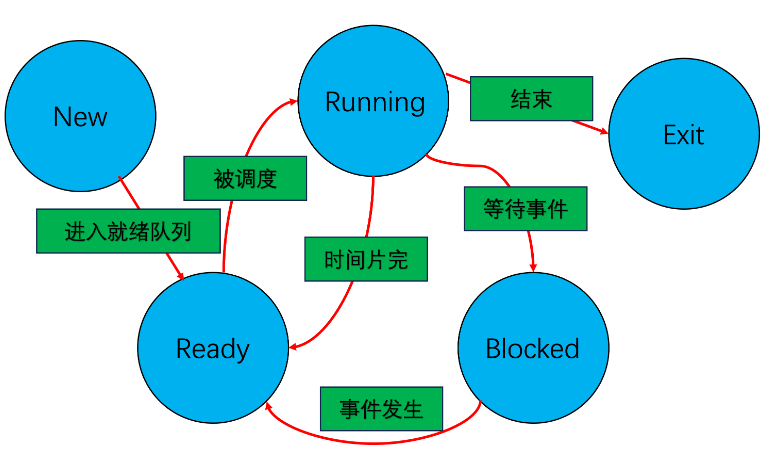
\includegraphics[width=1\linewidth]{figs\Proc.PNG}
    \caption{TCB结构示意图}
    \label{TCB结构示意图}
\end{figure}

如上述定义的TCB使得线程在 NPUcore-Impact!!! 中的理解变为了这样——一个可以与同线程组tg1d共享内存空间的进程即为线程.

\subsection{文件系统方面}

目前来讲,NPUcore-Impact!!!已经完美支持了fat32文件系统,正在积极的向ext4文件系统靠拢,对于fat32文件系统的描述,已在前几章详细讲过,这里不再详细描述.

\section{NPUcore-Impact!!!的优势}

\section{附件}
\subsection{附件1:内存常数一览}
\begin{center}
    \begin{lstlisting}[language=RUST,numbers=left]
pub const MEMORY_SIZE: usize = 0x1000_0000;
pub const USER_STACK_SIZE: usize = PAGE_SIZE * 40;
pub const USER_HEAP_SIZE: usize = PAGE_SIZE * 20;
pub const SYSTEM_TASK_LIMIT: usize = 128;
pub const DEFAULT_FD_LIMIT: usize = 128;
pub const SYSTEM_FD_LIMIT: usize = 256;
pub const PAGE_SIZE: usize = 0x1000;
pub const PAGE_SIZE_BITS: usize = PAGE_SIZE.trailing_zeros() as usize;
pub const PTE_WIDTH: usize = 8;
pub const PTE_WIDTH_BITS: usize = PTE_WIDTH.trailing_zeros() as usize;
pub const DIR_WIDTH: usize = PAGE_SIZE_BITS - PTE_WIDTH_BITS;
pub const DIRTY_WIDTH: usize = 0x100_0000;
#[cfg(debug_assertions)]
pub const KSTACK_PG_NUM_SHIFT: usize = 16usize.trailing_zeros() as usize;
#[cfg(not(debug_assertions))]
pub const KSTACK_PG_NUM_SHIFT: usize = 2usize.trailing_zeros() as usize;

pub const KERNEL_STACK_SIZE: usize = PAGE_SIZE << KSTACK_PG_NUM_SHIFT;
pub const KERNEL_HEAP_SIZE: usize = PAGE_SIZE * 0x3000;

// Addresses
/// Maximum length of a physical address
pub const PALEN: usize = 48;
/// Maximum length of a virtual address
pub const VALEN: usize = 48;
/// Maximum address in virtual address space.
/// May be used to extract virtual address from a segmented address
/// `0`-extension may be performed using this mask.
/// e.g. `flag` &= `VA_MASK`
pub const VA_MASK: usize = (1 << VALEN) - 1;
/// Mask for extracting segment number from usize address.
/// `1`-extension may be performed using this mask.
/// e.g. `flag` |= `SEG_MASK`
pub const SEG_MASK: usize = !VA_MASK;
/// Mask for extracting segment number from VPN.
/// All-one for segment field.
/// `1`-extension may be performed using this mask.
/// e.g. `flag` |= `SEG_MASK`
pub const VPN_SEG_MASK: usize = SEG_MASK >> PAGE_SIZE_BITS;

pub const HIGH_BASE_EIGHT: usize = 0x8000_0000_0000_0000;
pub const HIGH_BASE_ZERO: usize = 0x0000_0000_0000_0000;

// manually make usable memory space equal
pub const SUC_DMW_VESG: usize = 8;
pub const MEMORY_HIGH_BASE: usize = HIGH_BASE_ZERO;
pub const MEMORY_HIGH_BASE_VPN: usize = MEMORY_HIGH_BASE >> PAGE_SIZE_BITS;
pub const USER_STACK_BASE: usize = TASK_SIZE - PAGE_SIZE | LA_START;
pub const MEMORY_START: usize = 0x0000_0000_9000_0000;
pub const MEMORY_END: usize = MEMORY_SIZE + MEMORY_START;

pub const SV39_SPACE: usize = 1 << 39;
pub const USR_SPACE_LEN: usize = SV39_SPACE >> 2;
pub const LA_START: usize = 0x1_2000_0000;
pub const USR_VIRT_SPACE_END: usize = USR_SPACE_LEN - 1;
pub const TRAMPOLINE: usize = SIGNAL_TRAMPOLINE; // The trampoline is NOT mapped in LA.
pub const SIGNAL_TRAMPOLINE: usize = USR_VIRT_SPACE_END - PAGE_SIZE + 1;
pub const TRAP_CONTEXT_BASE: usize = SIGNAL_TRAMPOLINE - PAGE_SIZE;
pub const USR_MMAP_END: usize = TRAP_CONTEXT_BASE - PAGE_SIZE;
pub const USR_MMAP_BASE: usize = USR_MMAP_END - USR_SPACE_LEN / 8 + 0x3000;
pub const TASK_SIZE: usize = USR_MMAP_BASE - USR_SPACE_LEN / 8;
pub const ELF_DYN_BASE: usize = (((TASK_SIZE - LA_START) / 3 * 2) | LA_START) & (!(PAGE_SIZE - 1));

pub const MMAP_BASE: usize = 0xFFFF_FF80_0000_0000;
pub const MMAP_END: usize = 0xFFFF_FFFF_FFFF_0000;
pub const SKIP_NUM: usize = 1;

pub const DISK_IMAGE_BASE: usize = 0x800_0000 + MEMORY_START;
pub const BUFFER_CACHE_NUM: usize = 256 * 1024 * 1024 / 2048 * 4 / 2048;

pub static mut CLOCK_FREQ: usize = 0;
    \end{lstlisting}
\end{center}


\end{document}
